\chapter{Exercicis proposats}
\label{cap:exercicis-proposats}

\begin{exercici}
Expressa la relació de pertinença als conjunts $\mathbb{N}$, $%
\mathbb{Z}$, $\mathbb{Q}$ o $\mathbb{R}$ dels nombres següents:%
\[
\begin{array}{llllllll}
a) & 2/5 &  & b) & \sqrt{6} &  & c) & 2.87333... \\ 
&  &  &  &  &  &  &  \\ 
d) & 0.4142434... &  & e) & 3.1415926535... &  & f) & -7.832 \\ 
&  &  &  &  &  &  &  \\ 
g) & 5.272727... &  & h) & 5.000... &  & i) & \sqrt[5]{3}%
\end{array}%
\]

\end{exercici}

\begin{indicacio}
%
\[
\begin{array}{cccccc}
a) & \mathbb{Q} & b) & \mathbb{R} & c) & \mathbb{Q} \\ 
d) & \mathbb{R} & e) & \mathbb{R} & f) & \mathbb{Q} \\ 
g) & \mathbb{Q} & h) & \mathbb{N} & i) & \mathbb{R}%
\end{array}%
\]
\end{indicacio}

\begin{exercici}
Dels nombres reals següents, després d’efectuar les
operacions indicades, indica quins són racionals i quins no:%
\[
\begin{array}{llllllll}
a) & \sqrt[3]{-27} &  & b) & (1/5)^{1/2} &  & c) & \sqrt{100} \\ 
&  &  &  &  &  &  &  \\ 
d) & \left( \sqrt{3}\right) ^{0} &  & e) & 7^{-1} &  & f) & (-64)^{1/3} \\ 
&  &  &  &  &  &  &  \\ 
g) & (1/3)^{-1/2} &  & h) & (1/2)^{-1} &  & i) & \sqrt[4]{1/81}%
\end{array}%
\]

\end{exercici}

\begin{indicacio}
%
\[
\begin{array}{cccccc}
a) & -3\in \mathbb{Q} & b) & 1/\sqrt{5}\notin \mathbb{Q} & c) & 10\in 
\mathbb{Q} \\ 
d) & 1\in \mathbb{Q} & e) & 1/7\in \mathbb{Q} & f) & -4\in \mathbb{Q} \\ 
g) & \sqrt{3}\notin \mathbb{Q} & h) & 2\in \mathbb{Q} & i) & 1/3\in \mathbb{Q%
}%
\end{array}%
\]
\end{indicacio}

\begin{exercici}
Ordena de menor a major els nombres reals següents:%
\[
\begin{array}{cccccc}
-3/5 & 1.348125... & -1.8222... & -\sqrt{2} & \left\vert -5/3\right\vert & 
\frac{2}{5}%
\end{array}%
\]

\end{exercici}

\begin{indicacio}
%
\[
-1.8222...<-\sqrt{2}<-3/5<2/5<1.348125...<\left\vert -5/3\right\vert 
\]
\end{indicacio}

\begin{exercici}
Representa en la recta real els punts següents%
\[
\begin{array}{cccccc}
-\sqrt{2} & \sqrt{5} & -2\sqrt{5} & \sqrt{5}-1 & \sqrt{3} & 2\sqrt{3}-\sqrt{2%
}%
\end{array}%
\]%
i, després, ordena’ls de menor a major.

\end{exercici}

\begin{indicacio}
$-2\sqrt{5}<-\sqrt{2}<\sqrt{5}-1<\sqrt{3}<2\sqrt{3}-\sqrt{2}<%
\sqrt{5}$
\begin{center}
  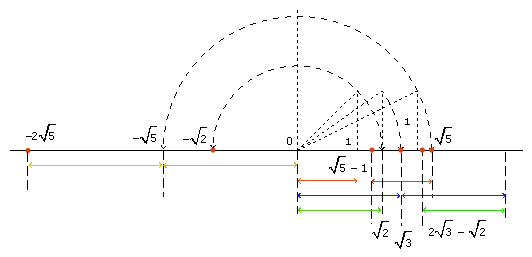
\includegraphics[width=5.5694in,height=2.7051in,keepaspectratio]{img/num66.png}
\end{center}
\end{indicacio}

\begin{exercici}
Forma les dues successions d’aproximacions successives per defecte i
per excés corresponents als nombres següents: (a) $7.28$, (b) $%
15.343434...$ i (c) $-2.357357357...$

\end{exercici}

\begin{indicacio}
(a)%
\[
\begin{array}{rccccc}
\text{defecte:} & 7 & 7.2 & 7.28 & 7.280 & \cdots \\ 
\text{excés:} & 8 & 7.3 & 7.29 & 7.281 & \cdots%
\end{array}%
\]%
(b)%
\[
\begin{array}{rccccc}
\text{defecte:} & 15 & 15.3 & 15.34 & 15.343 & \cdots \\ 
\text{excés:} & 16 & 15.4 & 15.35 & 15.344 & \cdots%
\end{array}%
\]%
(c)%
\[
\begin{array}{rccccc}
\text{defecte:} & -3 & -2.4 & -2.36 & -2.358 & \cdots \\ 
\text{excés:} & -2 & -2.3 & -2.35 & -2.357 & \cdots%
\end{array}%
\]
\end{indicacio}

\begin{exercici}
Troba una successió d’intervals encaixats que determini cadascun dels nombres reals següents: (a) $2.757575...$ (b) $%
3.2484848...$ i (c) $\pi $.

\end{exercici}

\begin{indicacio}
(a)%
\[
\lbrack 2,3]\supset \lbrack 2.7,2.8]\supset \lbrack 2.75,2.76]\supset
\lbrack 2.757,2.758]\supset \cdots 
\]%
(b)%
\[
\lbrack 3,4]\supset \lbrack 3.2,3.3]\supset \lbrack 3.24,3.25]\supset
\lbrack 3.248,3.249]\supset \cdots 
\]%
(c)%
\[
\lbrack 3,4]\supset \lbrack 3.1,3.2]\supset \lbrack 3.14,3.15]\supset
\lbrack 3.141,3.142]\supset \cdots 
\]
\end{indicacio}

\begin{exercici}
Escriu dues successions d’intervals encaixats que defineixin el nombre $2$.

\end{exercici}

\begin{indicacio}
%
\[
\lbrack 1,2]\supset \lbrack 1.9,2.0]\supset \lbrack 1.99,2.00]\supset
\lbrack 1.999,2.000]\supset \cdots 
\]%
\[
\lbrack 2,3]\supset \lbrack 2.0,2.1]\supset \lbrack 2.00,2.01]\supset
\lbrack 2.000,2.001]\supset \cdots 
\]
\end{indicacio}

\begin{exercici}
Troba tres nombres reals que estiguin compresos entre $%
1.342178...$ i $1.342179...$

\end{exercici}

\begin{indicacio}
Per exemple: $1.3421781$, $1.3421782$ i $1.3421783$
\end{indicacio}

\begin{exercici}
Calcula el valor de la diagonal d’un rectangle de costats $1$ i $%
\sqrt{2}$ i determina si és racional o irracional.

\end{exercici}

\begin{indicacio}
$\sqrt{3}$, que és un nombre irracional
\end{indicacio}

\begin{exercici}
A un rectangle d’altura $1$ i base el nombre auri $%
\frac{1+\sqrt{5}}{2}$ se li treu un quadrat de costat 1, i en resulta un altre rectangle. Troba les longituds dels costats d’aquest rectangle i
prova que és semblant al rectangle donat.

\end{exercici}

\begin{indicacio}
Les dimensions del rectangle són $\frac{\sqrt{5}-1}{2}$
i $1$. A més,%
\begin{align*}
\frac{1}{\frac{\sqrt{5}-1}{2}} &=\frac{2}{\sqrt{5}-1} \\
&=\frac{2(\sqrt{5}+1)}{(\sqrt{5}-1)(\sqrt{5}+1)} \\
&=\frac{\sqrt{5}+1}{2} \\
&=\frac{\frac{\sqrt{5}+1}{2}}{1}
\end{align*}
\end{indicacio}

\begin{exercici}
Suposant que $x=y$, en quin pas de la
següent deducció es comet l’error?%
\[
\begin{array}{cc}
(1) & x^{2}=xy \\ 
(2) & x^{2}-y^{2}=xy-y^{2} \\ 
(3) & (x+y)(x-y)=y(x-y) \\ 
(4) & x+y=y \\ 
(5) & 2y=y \\ 
(6) & 2=1%
\end{array}%
\]

\end{exercici}

\begin{indicacio}
En passar de (3) a (4) no es pot simplificar per $x-y$ ja que 
$x-y=0$
\end{indicacio}

\begin{exercici}
En una batalla han participat 4000 homes. Dels supervivents, el 
$56.\widehat{56}$ \% no fuma i el $56.\widehat{756}$ \% no beu. 
Quants homes han mort?

\end{exercici}

\begin{indicacio}
El nombre d’homes que han mort en la batalla és $337$
\end{indicacio}

\begin{exercici}
Troba tots els nombres reals $x$ tals que: (a) $x^{2}>3x+4$ i
(b) $1<x^{2}<4$.

\end{exercici}

\begin{indicacio}
(a) $(-\infty ,-1)\cup (4,+\infty )$ i (b) $(-2,-1)\cup (1,2)$
\end{indicacio}

\begin{exercici}
Resol les inequacions següents:

\begin{enumerate}
\item[a)] $\left\vert x+1\right\vert <2$

\item[b)] $\left\vert 2x-1\right\vert <\left\vert x-1\right\vert $

\item[c)] $\left\vert x+2\right\vert +\left\vert x-2\right\vert \leq 12$

\item[d)] $\left\vert \left\vert x+1\right\vert -\left\vert x-1\right\vert
\right\vert <1$
\end{enumerate}

\end{exercici}

\begin{indicacio}
(a) $(-3,1)$, (b) $(0,2/3)$, (c) $[-6,6]$ i (d) $(-1/2,1/2)$
\end{indicacio}

\begin{exercici}
Troba el suprem i l’ínfim dels subconjunts de nombres reals següents, indicant si són màxim o mínim respectivament.

\begin{enumerate}
\item[a)] $A=\left\{ x\in \mathbb{R}:0<x^{2}\leq 2\right\} $

\item[b)] $B=\left\{ \frac{1}{n}:n\in \mathbb{N}\right\} $

\item[c)] $C=\left\{ x\in \mathbb{R}:0<(x-2)^{2}\leq 3\right\} $

\item[d)] $D=\left\{ \frac{1}{3^{m}}:m\in \mathbb{Z}\right\} $
\end{enumerate}

\end{exercici}

\begin{indicacio}
%
\[
\begin{array}{ccccc}
\text{conjunt} & \sup & \inf & \max & \min \\ 
A & \sqrt{2} & -\sqrt{2} & \sqrt{2} & -\sqrt{2} \\ 
B & 1 & 0 & 1 & \text{No existeix} \\ 
C & 2+\sqrt{3} & 2-\sqrt{3} & 2+\sqrt{3} & 2-\sqrt{3} \\ 
D & \text{No existeix} & 0 & \text{No existeix} & \text{No existeix}%
\end{array}%
\]
\end{indicacio}

\begin{exercici}
Expressa en forma d’intervals els conjunts següents:

\begin{enumerate}
\item[a)] $A=\left\{ x\in \mathbb{R}:\left\vert x^{2}-2\right\vert \leq
1\right\} $

\item[b)] $B=\left\{ x\in \mathbb{R}:x^{2}+3x+3<1\right\} $

\item[c)] $C=\left\{ x\in \mathbb{R}:(x^{2}-x-1)/(x-1)>1\right\} $

\item[d)] $D=\left\{ x\in \mathbb{R}:\left\vert x-1\right\vert \left\vert
x+2\right\vert =3\right\} $
\end{enumerate}

\end{exercici}

\begin{indicacio}
%
\[
\begin{array}{l}
A=[-\sqrt{3},-1]\cup \lbrack 1,\sqrt{3}] \\ 
B=(-2,-1) \\ 
C=(0,1)\cup (2,+\infty ) \\ 
D=\left\{ \frac{-1-\sqrt{21}}{2},\frac{-1+\sqrt{21}}{2}\right\}%
\end{array}%
\]
\end{indicacio}

\begin{exercici}
Escriu el conjunt de punts que són a distància menor que $1/2$ de $5$.

\end{exercici}

\begin{indicacio}
$\left\{ x\in \mathbb{R}:d(x,5)<1/2\right\} =(9/2,11/2)$
\end{indicacio}

\begin{exercici}
Expressa en forma d’entorns els intervals següents%
\[
\begin{array}{cccccc}
a) & (-1,5) & b) & (0,3) & c) & (8,12)%
\end{array}%
\]

\end{exercici}

\begin{indicacio}
%
\[
\begin{array}{cccccc}
a) & E_{3}(2) & b) & E_{3/2}(3/2) & c) & E_{2}(10)%
\end{array}%
\]
\end{indicacio}

\begin{exercici}
Escriu en notació científica els nombres següents:
(a) $30^{4}$, (b) $(30000)^{-3}$ (c) $(0.025)^{2}$ i (d) $(4.56^{2})^{3}$

\end{exercici}

\begin{indicacio}
(a) $8.1\times 10^{5}$, (b) $3.7\times 10^{-14}$, (c) $%
6.25\times 10^{-4}$ i (d) $8.99\times 10^{3}$
\end{indicacio}

\begin{exercici}
Troba en cada cas el valor de $x$%
\[
\begin{array}{llllllll}
a) & \sqrt{x}=3 &  & b) & \sqrt[3]{x+1}=3 &  & c) & \sqrt[4]{5x-4}=2 \\ 
&  &  &  &  &  &  &  \\ 
d) & \sqrt[3]{x}+3=1 &  & e) & 3x^{3}+1=25 &  & f) & 1+\sqrt[3]{2x}=7%
\end{array}%
\]

\end{exercici}

\begin{indicacio}
%
\[
\begin{array}{cccccc}
a) & 9 & b) & 26 & c) & 4 \\ 
d) & -8 & e) & 2 & f) & 108%
\end{array}%
\]
\end{indicacio}

\begin{exercici}
Converteix en una sola arrel les expressions següents:%
\[
\begin{array}{llllllll}
a) & \sqrt[4]{2a^{2}b}\cdot \sqrt[4]{4ab^{2}} &  & b) & 5a^{2}\cdot \sqrt[4]{%
3a^{3}b^{2}} &  & c) & \frac{3\cdot \sqrt[3]{2a^{2}bc^{2}}\cdot \sqrt[3]{%
6a^{4}b^{2}}}{2a\cdot \sqrt[3]{ab^{4}c}} \\ 
&  &  &  &  &  &  &  \\ 
d) & \frac{\left( \sqrt[7]{a^{6}}\right) ^{2}\cdot \left( \sqrt[7]{a}\right)
^{5}}{a^{2}\cdot \left( \sqrt[7]{a}\right) ^{2}} &  & e) & a\cdot \left( 
\sqrt[3]{\sqrt[4]{a^{3}}}\right) ^{5} &  & f) & \sqrt[3]{4a^{2}}\cdot \sqrt[6%
]{2a}\cdot \sqrt[4]{4a} \\ 
&  &  &  &  &  &  &  \\ 
g) & \frac{\sqrt[4]{5a^{3}}\cdot \sqrt[6]{5a}}{\sqrt[3]{5a^{2}}\cdot \sqrt{a}%
} &  & h) & \sqrt{a^{2}\cdot \sqrt[4]{a\cdot \sqrt[5]{a}}} &  & i) & \frac{%
\sqrt[5]{a^{2}\cdot \sqrt[3]{b^{-8}\cdot a^{-4}}}}{\sqrt[4]{a^{-2}\cdot
b^{3}\cdot \sqrt[3]{a^{5}\cdot b^{4}}}}%
\end{array}%
\]

\end{exercici}

\begin{indicacio}
%
\[
\begin{array}{cccccc}
a) & \sqrt[4]{8a^{3}b^{3}} & b) & \sqrt[4]{1875a^{11}b^{2}} & c) & \sqrt[3]{%
\frac{81a^{2}c}{2b}} \\ 
d) & \sqrt[7]{a} & e) & \sqrt[4]{a^{9}} & f) & \sqrt[12]{65536a^{13}} \\ 
g) & \sqrt[12]{\frac{5}{a^{3}}} & h) & \sqrt[20]{a^{23}} & i) & \sqrt[60]{%
\frac{a^{13}}{b^{97}}}%
\end{array}%
\]
\end{indicacio}

\begin{exercici}
Simplifica les arrels següents:%
\[
\begin{array}{llllllll}
a) & \sqrt[3]{2592\cdot a^{11}\cdot b^{23}\cdot c^{102}} &  & b) & \sqrt[3]{%
\frac{864a^{7}b^{2}}{625d^{9}c^{112}}} &  & c) & \frac{\sqrt[5]{81a^{4}b^{3}}%
}{\sqrt[5]{27a^{3}b^{4}}} \\ 
&  &  &  &  &  &  &  \\ 
d) & \sqrt[4]{4a^{3}x^{2}}\cdot \sqrt[4]{72ax^{2}}\cdot \sqrt[4]{18a^{2}x} & 
& e) & \sqrt[4]{125\cdot \sqrt{625\cdot \sqrt[5]{25}}} &  & f) & \sqrt[3]{%
\frac{\sqrt[3]{25}\cdot \sqrt[5]{5}}{\sqrt[3]{5}\cdot \sqrt[4]{125}}}%
\end{array}%
\]

\end{exercici}

\begin{indicacio}
%
\[
\begin{array}{cccccc}
a) & 6a^{3}b^{7}c^{34}\sqrt[3]{12a^{2}b^{2}} & b) & \frac{6a^{2}}{%
5d^{3}c^{37}}\sqrt[3]{\frac{4ab^{2}}{5c}} & c) & \sqrt[5]{\frac{3a}{b}} \\ 
d) & 6ax\cdot \sqrt[4]{4a^{2}x} & e) & 5\sqrt[10]{125} & f) & \sqrt[180]{%
1/5^{13}}%
\end{array}%
\]
\end{indicacio}

\begin{exercici}
Simplifica les expressions següents:

\begin{enumerate}
\item[a)] $\sqrt{343}+\sqrt{48}+\sqrt{\frac{28}{81}}+\sqrt{\frac{300}{121}}$

\item[b)] $\sqrt{125}-3\sqrt{80}-4\sqrt{45}+10\sqrt{180}$

\item[c)] $\sqrt[3]{\frac{81}{8}}-\sqrt[3]{\frac{375}{64}}+\sqrt[3]{\frac{81%
}{125}}$

\item[d)] $(3\sqrt{2}-2\sqrt{3})\cdot (\sqrt{2}+\sqrt{3})-(2-\sqrt{6})^{2}$

\item[e)] $(3+\sqrt{5})^{2}-3(2\sqrt{5}-3)^{2}$
\end{enumerate}

\end{exercici}

\begin{indicacio}
%
\[
\begin{array}{ll}
a) & \frac{65}{9}\sqrt{7}+\frac{54}{11}\sqrt{3} \\ 
b) & 65\sqrt{5} \\ 
c) & \frac{17}{20}\sqrt[3]{3} \\ 
d) & 5\sqrt{6}-10 \\ 
e) & 42\sqrt{5}-73%
\end{array}%
\]
\end{indicacio}

\begin{exercici}
Racionalitza el denominador de les expressions següents:%
\[
\begin{array}{llllllll}
a) & \frac{14\sqrt{5}}{\sqrt[3]{7}} &  & b) & \frac{3\sqrt{2}}{\sqrt{18}} & 
& c) & \frac{5\sqrt{3}+\sqrt{12}}{14\sqrt{3}} \\ 
&  &  &  &  &  &  &  \\ 
d) & \frac{6\sqrt{5}}{\sqrt[4]{3}} &  & e) & \frac{1}{\sqrt[3]{8a^{2}}} &  & 
f) & \frac{6ab}{\sqrt[4]{288a^{2}b^{5}}} \\ 
&  &  &  &  &  &  &  \\ 
g) & \frac{a}{\sqrt{2a+1}} &  & h) & \frac{a^{2}-b^{2}}{\sqrt{a+b}} &  & i)
& \frac{1+x}{\sqrt{1-x^{2}}}%
\end{array}%
\]

\end{exercici}

\begin{indicacio}
%
\[
\begin{array}{cccccc}
a) & 2\sqrt{5}\cdot \sqrt[3]{49} & b) & 1 & c) & 1/2 \\ 
d) & 2\sqrt{5}\cdot \sqrt[4]{27} & e) & \frac{\sqrt[3]{a}}{2a} & f) & \frac{%
\sqrt[4]{72a^{2}b^{3}}}{2b} \\ 
g) & \frac{a\sqrt{2a+1}}{2a+1} & h) & (a-b)\sqrt{a+b} & i) & \frac{\sqrt{%
1-x^{2}}}{1-x}%
\end{array}%
\]
\end{indicacio}

\begin{exercici}
Racionalitza el denominador de les expressions següents:

\begin{enumerate}
\item[a)] 
\[
\frac{1}{\sqrt{3}+\sqrt{2}} 
\]

\item[b)] 
\[
\frac{\sqrt{2}}{3-\sqrt{2}} 
\]

\item[c)] 
\[
\frac{\sqrt{3}+\sqrt{2}}{\sqrt{3}-\sqrt{2}} 
\]

\item[d)] 
\[
\frac{(3\sqrt{2}-1)(\sqrt{2}+1)}{\sqrt{2}-1} 
\]

\item[e)] 
\[
\frac{3+4\sqrt{3}}{\sqrt{6}+\sqrt{2}-\sqrt{5}} 
\]

\item[f)] 
\[
\frac{1}{\sqrt{3-\sqrt{3}}} 
\]
\end{enumerate}

\end{exercici}

\begin{indicacio}
%
\[
\begin{array}{ll}
a) & \sqrt{3}-\sqrt{2} \\ 
b) & \frac{3\sqrt{2}+2}{7} \\ 
c) & 5+2\sqrt{6} \\ 
d) & 7\sqrt{2}+9 \\ 
e) & \sqrt{6}+\sqrt{2}+\sqrt{5} \\ 
f) & \frac{1}{6}(3+\sqrt{3})\sqrt{3-\sqrt{3}}%
\end{array}%
\]
\end{indicacio}

\begin{exercici}
Opera i simplifica en les expressions següents:

\begin{enumerate}
\item[a)] 
\[
\frac{5-\sqrt{5}}{5+\sqrt{5}}-\frac{5+\sqrt{5}}{5-\sqrt{5}}+\frac{5}{\sqrt{5}%
} 
\]

\item[b)] 
\[
\frac{1+\sqrt{15}}{(\sqrt{5}-\sqrt{3})^{2}}+\frac{1-\sqrt{15}}{(\sqrt{5}+%
\sqrt{3})^{2}} 
\]

\item[c)] 
\[
\frac{2+\sqrt{2}}{\sqrt{3}-1}-\frac{\sqrt{3}-1}{2+\sqrt{2}}-2 
\]
\end{enumerate}

\end{exercici}

\begin{indicacio}
%
\[
\begin{array}{cc}
a) & 0 \\ 
b) & 19 \\ 
c) & \sqrt{6}%
\end{array}%
\]
\end{indicacio}

\begin{exercici}
Simplifica les expressions següents:

\begin{enumerate}
\item[a)] 
\[
\sqrt{a+b+\sqrt{2ab}}\cdot \sqrt{a+b-\sqrt{2ab}} 
\]

\item[b)] 
\[
\sqrt{1-2\sqrt{x}+x} 
\]

\item[c)] 
\[
\sqrt{192(x+1)^{4}(x-9)^{2}} 
\]

\item[d)] 
\[
\sqrt{\frac{a-b}{(a+b)^{2}}}\cdot \sqrt{\frac{a+b}{a^{2}-b^{2}}} 
\]

\item[e)] 
\[
\sqrt{4a^{2}+12ab+9b^{2}} 
\]
\end{enumerate}

\end{exercici}

\begin{indicacio}
%
\[
\begin{array}{ll}
a) & \sqrt{a^{2}+b^{2}} \\ 
b) & 1-\sqrt{x} \\ 
c) & 8\sqrt{3}\cdot (x+1)^{2}\cdot (x-9) \\ 
d) & \frac{1}{a+b} \\ 
e) & 2a+3b%
\end{array}%
\]
\end{indicacio}

\begin{exercici}
Calcula les expressions següents:%
\[
\begin{array}{llllllll}
a) & 16^{0.25} &  & b) & 4^{-3/2} &  & c) & \sqrt[11]{\frac{9}{27^{-3}}} \\ 
&  &  &  &  &  &  &  \\ 
d) & \left( \sqrt{27}\cdot 27^{-5/3}\right) ^{1/3} &  & e) & 0.0064^{1/2} & 
& f) & 2\sqrt{\frac{1}{2}\sqrt{\frac{1}{2}\sqrt{\frac{1}{2}\sqrt{\frac{1}{2}}%
}}} \\ 
&  &  &  &  &  &  &  \\ 
g) & \left[ \left( a^{-4}\right) ^{1/3}\cdot \left( a^{2}\right) ^{2/3}%
\right] :\left( a^{-3}\right) ^{1/3} &  & h) & \left[ \left( a^{1/4}\right)
^{3}\right] ^{-4/3} &  & i) & \left( a^{-4}\right) ^{1/3}\cdot \left(
a^{2}\right) ^{2/3}\cdot a^{-3}%
\end{array}%
\]

\end{exercici}

\begin{indicacio}
%
\[
\begin{array}{cccccc}
a) & 2 & b) & 1/8 & c) & 3 \\ 
d) & 3^{-7/6} & e) & 2/25 & f) & \sqrt[16]{2} \\ 
g) & a & h) & 1/a & i) & 1/a^{3}%
\end{array}%
\]
\end{indicacio}
